
\section{Greifen}

\begin{frame}[b]
	\begin{figure}
		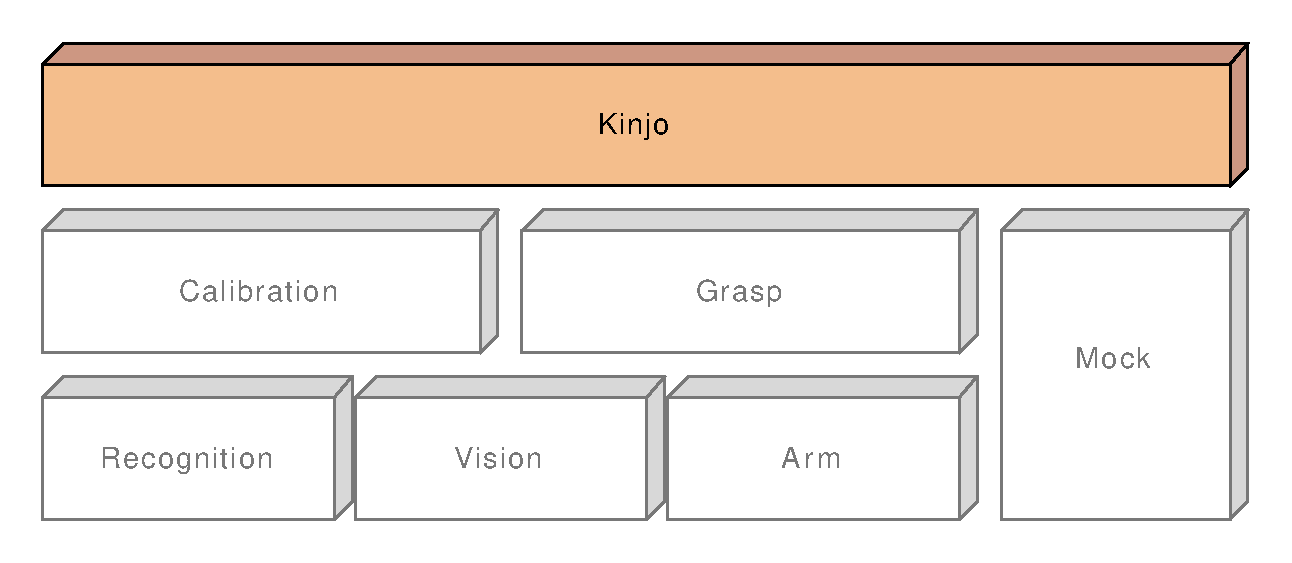
\includegraphics[width=0.8\textwidth]{nav_kinjo}
	\end{figure}
	\vspace*{0.7cm}
\end{frame}

\section{Ausblick}

\begin{frame}{Ausblick}
	\begin{block}{Bisherige Ergebnisse}
		\begin{itemize}
			\item Grundlegende Programmarchitektur
			\item Positionierung des Arms und Erkennung des
				Kalibrierungsobjektes
			\item Starrkörpertransformation (\emph{noch} fehlerbehaftet)
			\item Evaluation der Armgenauigkeit
			\item Mock-Implementation zum Testen ohne Geräte
		\end{itemize}
	\end{block}
	\begin{block}{Ausstehende Ergebnisse}
		\begin{itemize}
			\item Fehlerbehebung bei der Starrkörpertransformation
			\item Algorithmus zum Greifen des Objektes
			\item Anpassung der bisherigen \enquote{GUI} für bessere
				Bedienbarkeit
		\end{itemize}
	\end{block}
\end{frame}

